\chapter{Integrazione numerica}
\section{Quadratura dei trapezi}
La quadratura dei trapezi è un metodo di integrazione numerica che permette di approssimare il valore di un integrale definito. Il metodo consiste nell'approssimare l'area sottesa alla curva della funzione integranda con quella di un trapezio avente come basi i valori della funzione nei due estremi dell'intervallo di integrazione e come altezza la lunghezza dell'intervallo stesso diviso il numero di sottointervalli in cui si vuole suddividere l'intervallo di integrazione.
\begin{align}
  T_N(f) = \frac{b - a}{2 N} [ f(a) + 2 \sum_{i=1}^{N-1} f(x_i) + f(b) ]
\end{align}

Nel caso semplice dove $N = 1$ si ha:
\begin{align}
  T(f) = \frac{b - a}{2} [ f(a) + f(b) ]
\end{align}

$N$ rappresenta il numero di sottointervalli in cui si suddivide l'intervallo di integrazione. Quindi, per $N = 1$ si ha un solo sottointervallo, mentre per $N = 2$ si hanno due sottointervalli e così via.



\subsection{Errore di quadratura}
Il resto di quadratura per i trapezi è:
\begin{align}
  r(T_N) &= I(f) - T_N(f) \\
  &= - \frac{1}{12} \frac{(b - a)^3}{N^2} f''(\xi)
\end{align}


\begin{figure}[h!]
  \centering
  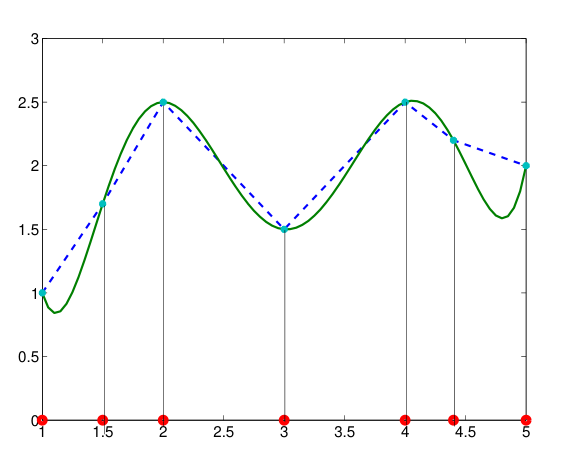
\includegraphics[width=0.4\linewidth]{./images/trapezi}
\end{figure}


\section{Quadratura di Cavalieri-Simpson}

A differenza della quadratura dei trapezi dove si utilizzazvano delle dei segmenti per interpolare i vari punti dell'intervallo,
con cavaliaeri-simpson si utilizzano delle parabole. In questo modo si riesce ad ottenere una maggiore precisione.

\begin{align}
  \int_a^b f(x) dx \approx \frac{b - a}{6N} \Bigg[ f(a) + 2 \sum_{i=1}^{N-1} f(x_i) + 4 \sum_{i=1}^{N-1} f(\frac{x_i + x_{i+1}}{2}) + f(b) \Bigg]
\end{align}

\subsection{Errore di quadratura}
Il resto di quadratura per la quadratura di Cavalieri-Simpson è:
\begin{align}
  r{CS_N} &= I(f) - CS_N(f) \\
  &= - \frac{(b - a)^5}{2880N} f^{(4)}(\xi)
\end{align}



\section{Grado di precisione}
Una formula di quadratura ha grado di precisione $d$ se \`e esatta quando $f(x)$ \`e polinomio qualsiasi di grado $\leq d$ 
ed esiste almeno un polinomio di grado $d+1$ dove $err\neq 0$.


\begin{center}
  \begin{tabular}{| c | c |}
    \hline
    Trapezi & $d \leq 1$ \\
    Cavalieri-Simpson & $d \leq 3$ \\
    \hline
  \end{tabular}
\end{center}

\renewcommand{\arraystretch}{1.4}

\section{Coefficiente di Newton-Cotes}
\begin{center}
  \begin{tabular}{| c | c | c | c | c | c |}
    \hline
    n & $\alpha_0$ & $\alpha_1$ & $\alpha_2$ & $\alpha_3$ & resto \\
    \hline
    1 & $\frac{1}{2}$ & $\frac{1}{2}$ & & & $-\frac{1}{12}h^3f^{(2)}(\xi)$ \\
    \hline
    2 & $\frac{1}{3}$ & $\frac{4}{3}$ & & & $-\frac{1}{90}h^5f^{(4)}(\xi)$ \\
    \hline
    3 & $\frac{3}{8}$ & $\frac{9}{8}$ & & & $-\frac{3}{80}h^5f^{(4)}(\xi)$ \\
    \hline
    4 & $\frac{14}{45}$ & $\frac{64}{45}$ & $\frac{24}{45}$ & & $-\frac{8}{945}h^7f^{(6)}(\xi)$ \\
    \hline
    5 & $\frac{95}{288}$ & $\frac{375}{288}$ & $\frac{250}{288}$ & & $-\frac{275}{12096}h^7f^{(6)}(\xi)$ \\
    \hline
    6 & $\frac{41}{140}$ & $\frac{216}{140}$ & $\frac{27}{140}$ & $\frac{272}{140}$ & $-\frac{9}{1400}h^9f^{(8)}(\xi)$ \\
    \hline
    7 & $\frac{5257}{17280}$ & $\frac{25039}{17280}$ & $\frac{9261}{17280}$ & $\frac{20926}{17280}$ & $-\frac{8183}{518400}h^9f^{(8)}(\xi)$ \\
    \hline
  \end{tabular}
\end{center}

